%!TEX root = ../main.tex
\section{Introduction}
For this master thesis, we wanted to be able to analyse the difference between several data structures. Moreover, willing to work with big graph, the traditional adjacency matrix became too heavy and the access time was too low. As a reminder, a adjacency matrix is two dimension array, where each line represents a starting node and each column represents a ending node. The values represent the capacity between both nodes, 0 meaning that there are no edge between them. \newline

\begin{figure}[!h]
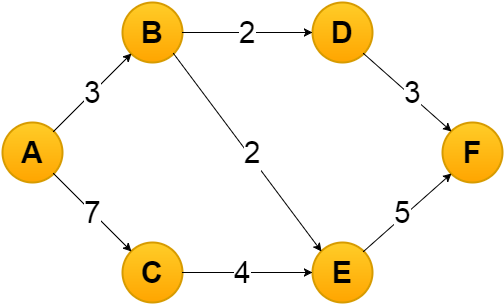
\includegraphics[width=7.5cm,height=4.5cm]{images/graph.png}
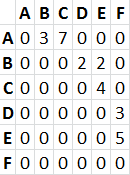
\includegraphics[scale=0.7]{images/adjacencyMatrix.png}
\caption{A graph with its adjacency matrix}
\end{figure}

TODO Voir avec Denis comment mettre cette table mieux \newline


So we decide to use a structure defined below. \newline

Like for the adjacency matrix, we use a array where each line represents the neighbours of a node. For example, the first line contains the information on the neighbours of the node 0. But contrary to the adjacency matrix, we do not use a array to represent neighbours but a different structure requiring less memory space. \newline

We used four various data structures : hash map, tree map, simple linked list and one home-made structure, split array. Each node will have its structure, storing which nodes are neighbours and what are the capacities of the edges to these nodes. If we had to represent a graph with 10 nodes, we would have a array of 10, for example, hash map. Each hash map representing the neighbourhood of a single node.

\section{Data structures}
\subsection{Hash Map}
A hash map is an unordered associative array, associates a key with a value, so use as little space as possible. It contains an single array of buckets, where the values are stored. A hash function converts the key into index, which represents the bucket where the record (key/value) is stored. \newline

Ideally, the hash function assigns to every key a different bucket but it is possible to have several keys giving the same hash code. This is called a \textit{collision}. The bucket can thus contain several records. \newline

The \textit{load factor} is the number of records divided by the number of buckets.  The more the load factor is high, the more the hash map is slow. But having a too low load factor does not save search time, it just uses some memory pointlessly. To keep the load factor to a defined value (eg between $2/3$ and $3/4$), we must, when inserting new records, resize the hash map. \newline

In our case, the key is the id of the nearby node and the value is the capacity of the edge.

\subsection{Tree Map}
A tree map, or Red-Black tree, is a self-balancing binary search tree. In addition to the restrictions imposed by the binary search tree, which is to have for each node, the \textit{left} sub-tree containing only lower keys and the \textit{right} sub-tree only higher keys, the Red-Black tree respects four other conditions thanks to an additional information, the color of a node :

\begin{itemize}
\item A node is either red or black
\item The root is black
\item The parent of a red node is black
\item For each leaf, the path to the root contains the same number of black nodes
\end{itemize}

These constraints imply an important property of the Red-Black trees : the longest possible path from a root to a leaf can be only twice as long as the smallest possible. We thus have an almost balanced tree.

\begin{center}
\includegraphics[scale=0.4]{images/Red-Blacktree.png}
\captionof{figure}{A Red-Black tree}
\end{center}

\subsection{Simple Linked List}
A simple linked list is one of the simplest data structure. Each node consists of two fields, a data and a reference to the next node. It's unordered.

\subsection{Split Array}
A split array is a simplified version of a sparse set. It contains a single array of all possible neighbouring nodes (forward and backward edges). The array is divided into two parts, one with the current neighbour nodes (forward edges) and the other one with the nodes which are not, or no more, neighbours (backward edges). An integer value \textit{split} indicates the position of the array's separation.

\begin{figure}[!h]
\includegraphics[width=7.5cm,height=4.5cm]{images/SplitArrayGraph.png}\hfill
\includegraphics[width=5cm,height=3cm]{images/SplitArray.png}
\caption{A graph with the split array of node 2}
\end{figure}

To add a node (for example after sending units of flow on the path 0-1-2-4-5, an edge is created from 2 to 1 and 1 becomes a current neighbour of 2), we need to go through the right part of the array to find the futur neighbour node, exchange its place with the node on the right of \textit{split} and increase \textit{split} by 1. \newline

To remove a node, it's the reverse operation.


\subsection{Complexities}

This table below represents the complexities with the notation big O, what it means "in the worst case". Although for the last 3 structures, the worst case is not too penalizing but that is not the case for the hash map. Indeed, we obtain $O(n)$ if every elements of the hash map are in the same bucket. However, with a correct hash function, it should not arrive. \newline

\begin{tabular}{|c|c|c|c|c|}
	\hline
     & \textbf{Hash map} & \textbf{Tree map} & \textbf{Simple linked list} & \textbf{Split Array} \\
     \hline	
   entrySet & $O(n)$ & $O(n)$ & $O(n$) & $O(n)$\\
   get/set & $O(n)$ & $O(log$ $n)$ & $O(n)$ & $O(n)$\\
   put & $O(n)$ & $O(log$ $n)$ & $O(1)$ & $O(n^-)$\\
   remove & $O(n)$ & $O(log$ $n)$ & $O(n)$ & $O(n)$\\
   \hline
\end{tabular} \newline
with $n$ the number of forward edges of a node and $n^-$ the number of backward edges. So, $n$ is also the number of neighbours.